\title{Ueberschrift}%%TODO
\author{Wenwen Chen, Christian Dietz, \\
	Jan Seeger, Rainer Schoenberger, Julian Tatsch
}
\date{\today}

\documentclass[12pt]{article}
\usepackage{graphicx}

\begin{document}
\maketitle

\begin{abstract}
%%TODO
\end{abstract}

\section{Introduction}

overview
architecture bild

\section{Simulator}


After staring up the simulator, the car can be driven via the arrow keys. When pressing \textit{C}, one can delegate the control to the built-in TCP server. The current state is shown in the upper left corner.
When the control mode is switched to \textit{TCP}, the simulator accepts commands via TCP/IP.
The TCP/IP interface accepts the same commands as the servoboard.
In this way, the RaspberryPi can be attached to the simulator instead of the real car.
Also, the simulator does not have to run on the same machine as the control software.
So for example, the RaspberryPi can be mounted on the car, but for testing purposes send the commands to the simulator instead of the servoboard.

In addition to a very simple physical driving model, the simulator also simulates the output, which would be given by our concept of a laser scanner. This output can be seen in the rectangle in the top of the simulator window. The red lines in front of the car depict the viewing angle of the camera, which is used for the laser scanner.

A screenshot of the simulator can be seen in Figure \ref{figsim}.

\begin{figure}[h]
\begin{center}
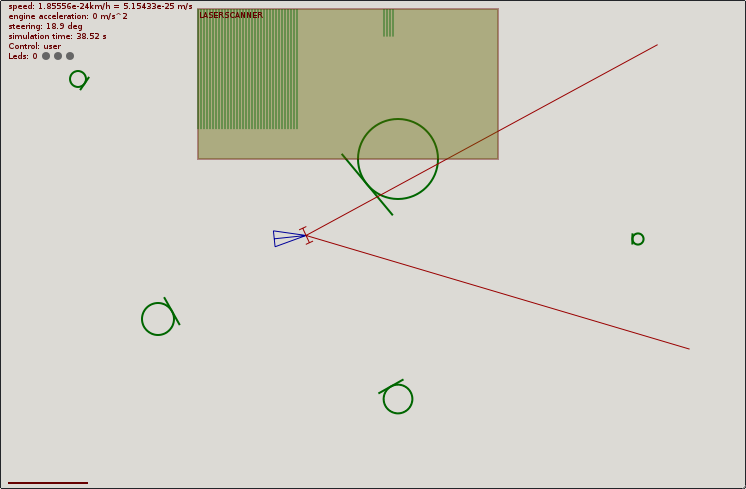
\includegraphics[width=15cm]{pic/sim.png}
\caption{Simulator}
\end{center}
\label{figsim}
\end{figure}

\section{RaspberryPi}
The RaspberryPi is used for highlevel communication.
It is connected to a wifi module via USB and opens up an access point.
The RasPi is also equipped with a bluetooth module to commuticate with a Wiimote controller.

\subsection{Software}
On the RaspberryPi, there runs the raspi.exe program, which can be found in the \textit{raspi} folder.
It will start up a TCP/IP server and listen for a Wiimote controller via bluetooth.
Over those interfaces, it will accept highlevel commands to control the car.
Note that only one device is able to control the car at a time.
There is a handover mechanism implemented in the \textit{raspi.exe} program: If a device sends a \textit{getperm}-command, it will take over the control and commands from other currently connected devices are ignored.


The configuration of the raspi.exe program is done via the file \textit{config.h}:
SERVO\_M defines, to which module the raspi software will send its commands. The possible values are:
\begin{itemize}
\item{SERVO\_SIM}
\item{SERVO\_BOARD}
\item{SERVO\_FPGA}
\end{itemize}

If SERVO\_SIM is set, \textit{raspi.exe} will send the commands to a simulation program via TCP/IP.
The IP and TCP port of the simulation program can also be configured in the \textit{config.h} file.
The \textit{raspi.exe} will send its commands directly to the servoboard via I2C, if SERVO\_M is set to SERVO\_BOARD.
The last option SERVO\_FPGA causes \textit{raspi.exe} to talk to the FPGA board via SPI.

If a Wiimote controller should be used to control the car, WII\_ENABLED must be set to 1 in the \textit{config.h} file.
Communication via TCP/IP is always enabled.

Settings, which are more specific to one communication unit, can be configured in \textit{servoboard.h, servosim.h} or \textit{fpga\_spi.h} respectively. Those files contain the parameters for the I2C or SPI specific communication, such as addresses, speeds or the paths to the chardevs.

\subsection{TCP communication protocol}
The \textit{raspi.exe} TCP server accepts the following commands:
\begin{description}
\item[servo set $<$channel$>$ $<$valve$>$] Sets the servo which is connected on PIN $<$channel$>$ to the corresponding value. $<$channel$>$ must be an integer between 0 and 7. $<$value$>$ is also an integer. It can have values from 0 to 8000, where 4000 would mean the zero position.
\item[servo led $<$onoff$>$ $<$mask$>$] Sets the LEDs on the servoboard. $<$onoff$>$ decides, wether the LEDs should be switched on(1) or off(0). The the three LSBs of $<$mask$>$ decide, which LEDs should be switched. Only LEDs, where the bit in the mask is set to 1 will be switched on or off. For example, if one wants to enable the first and the third LED, one would send the command "servo led 1 5". Note that most of the LEDs are by default also used by the servoboard firmware to signal various events. Once a LED has been manually set to a certain state by setting a bit to one in $<$mask$>$, this LED will not be used by the firmware anymore.
\item[servo getperm] This command initiates an control handover to the device, which is sending this command. From now on, \textit{raspi.exe} will only accept control commands from this device. All other currently connected devices will be ignored.
\item[speedv set $<$speed$>$ $<$steering$>$] This is a highlevel command, which is only accepted, if the Raspi is connected to the fpga. $<$speed$>$ and $<$steering$>$ are both double values.
\end{description}

\section{Servo controller board}
%%TODO: bildchen

%%TODO: servo-parameter (0-4000-8000)
\subsection{Schematics}

\begin{figure}[h]
\begin{center}
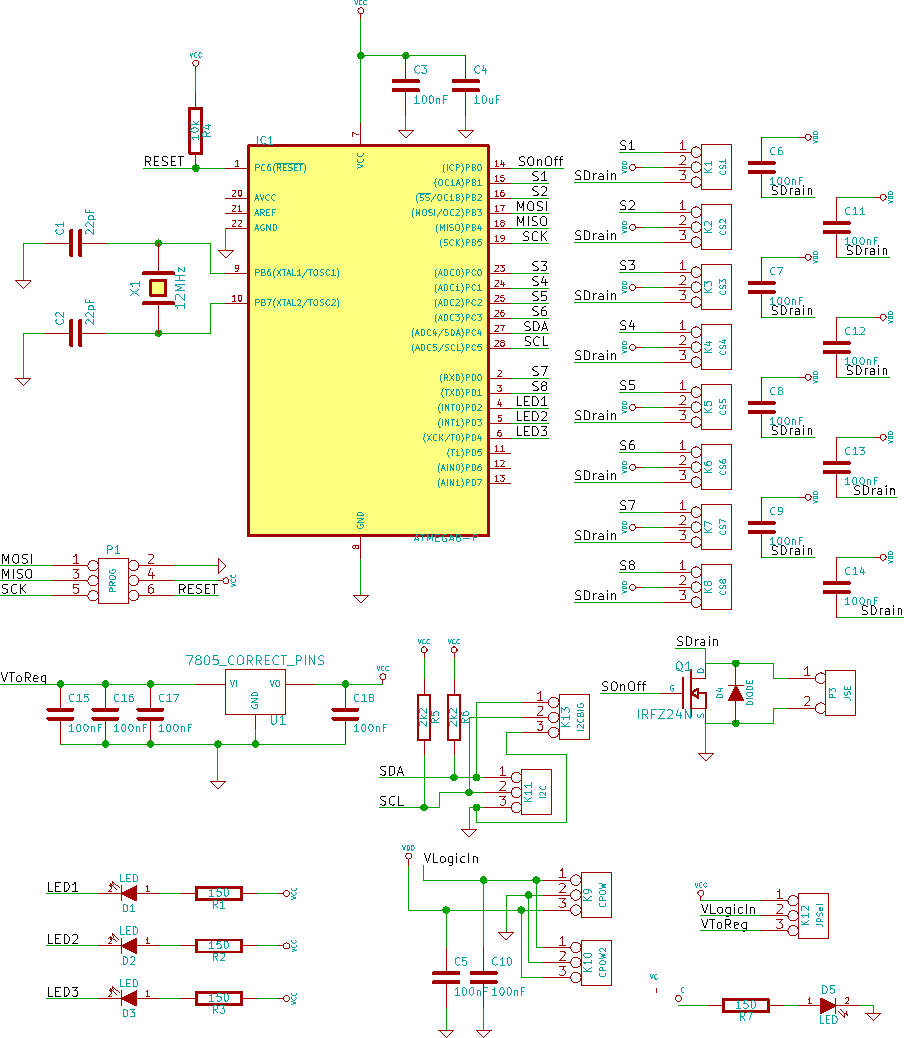
\includegraphics[width=20cm,angle=-90]{pic/servoboard}
\caption{Servoboard schematics}
\end{center}
\label{figservoboardscm}
\end{figure}

\subsection{Board}
After the schematics have been created, the PCB board layout was designed.
The components are placed on the board and connected with the corresponding copper tracks.
This process is also called routing.
Routing wasn't a big problem, as we had enough room on the board.
Almost all tracks fitted on one layer and only a few vias and additional floating wires were needed.
This made the PCB manufacturing process easier, as only a one-sided PCB could be used.
Figure \ref{figservoboardbrd} shows the finished board layout, Figure \ref{figservoboard3d} shows a 3D rendering of the servoboard and the finished board can be seen in Figure \ref{figservoboardr}.


\begin{figure}[h]
\begin{center}
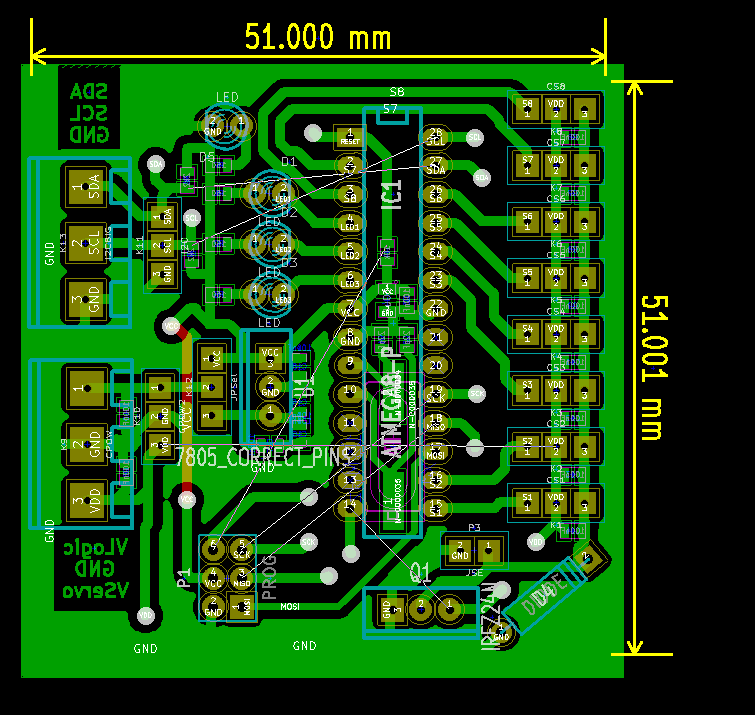
\includegraphics[width=5cm]{pic/servoboardbrd.png}
\caption{Servoboard}
\end{center}
\label{figservoboardbrd}
\end{figure}

\begin{figure}[h]
\begin{center}
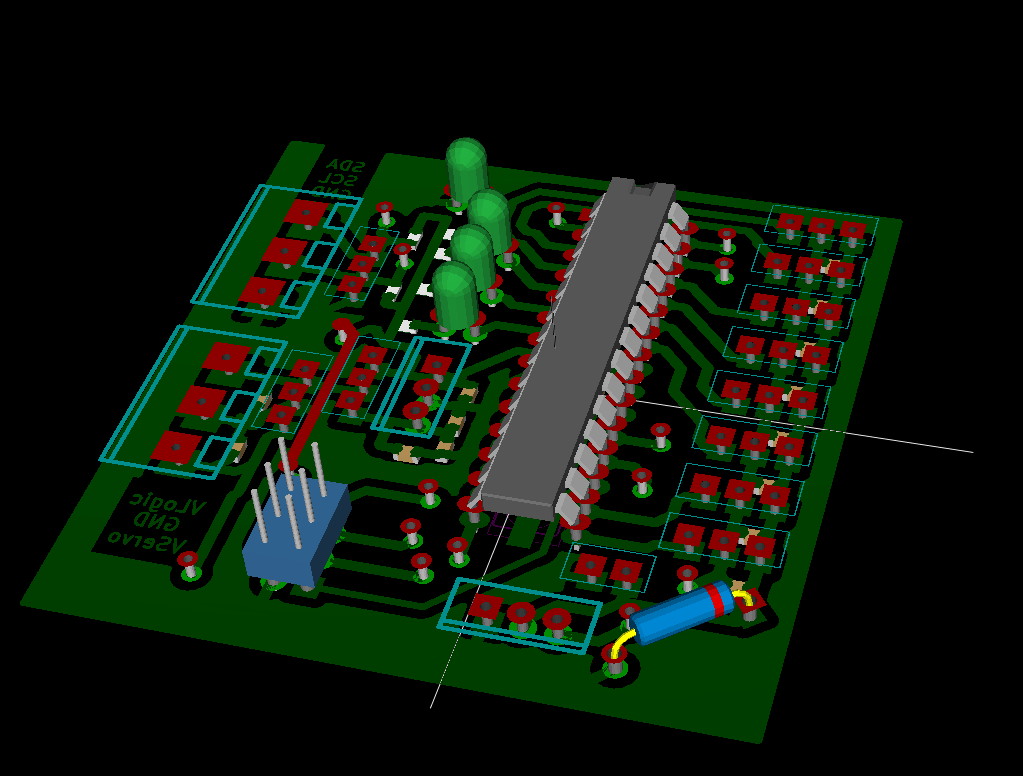
\includegraphics[width=5cm]{pic/servoboard3d.png}
\caption{Servoboard}
\end{center}
\label{figservoboard3d}
\end{figure}

\begin{figure}[h]
\begin{center}
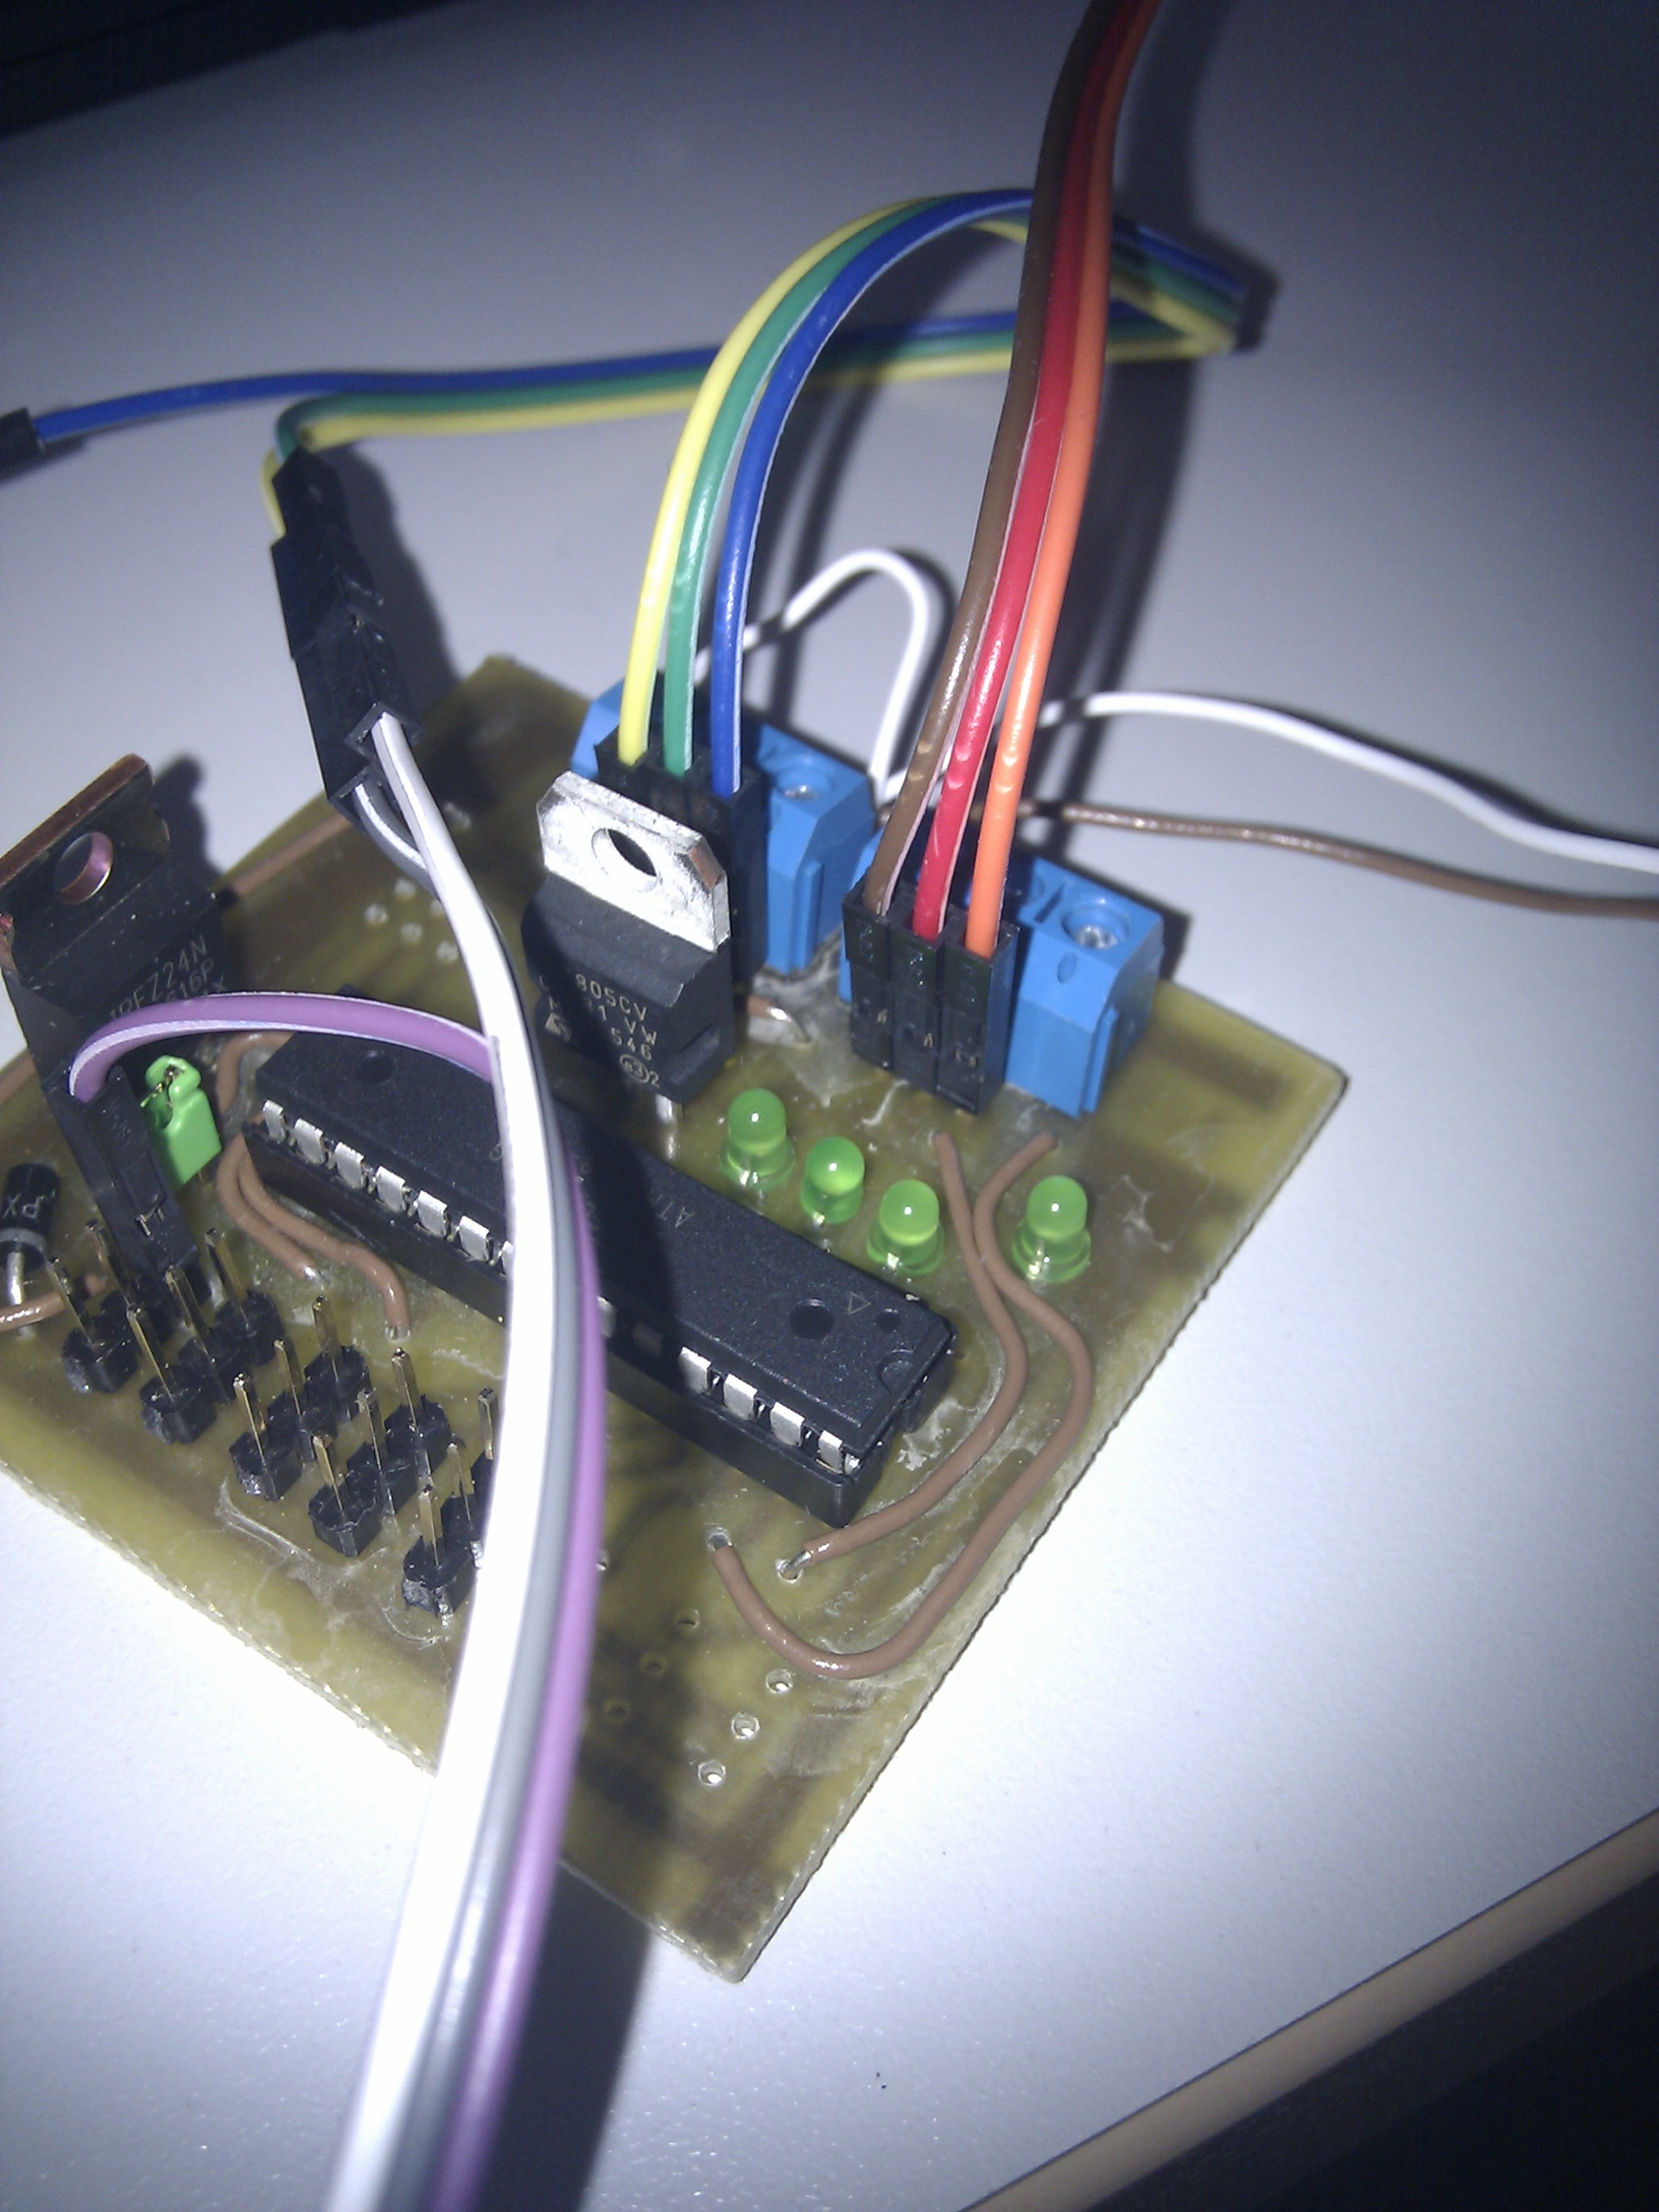
\includegraphics[width=5cm]{pic/servoboardr.jpg}
\caption{Servoboard}
\end{center}
\label{figservoboardr}
\end{figure}

\subsection{Communication protocol}
The Servoboard is connected via the I2C or two-wire interface to a command unit.
The command unit can either be the FPGA or the RaspberryPi.


The I2C protocol is not implemented in software, but the hardware I2C capabilities of the AVR Atmega8 microcontroller are used.
This gives us faster response time and less overhead.
It also unburdens the AVR CPU, as only one hardware interrupt is needed, each time a complede byte is received via I2C.
Implementing I2C via software would have required many timer interrupts and might have turned out less stable.


We implemented our own communication protocol ontop of I2C.
In the microcontroller's firmware, we used a simple state machine to realize this.

The communication protocol looks as follows:
The Master first sends a preamble (0xff), which is used to synchronize both communication partners.
This is necessary, because loosing packets or receiving corrupted data can lead to a situation, where the receiving unit ends up in an undefined or faulty state.
Therefore, it might be that the communication gets stuck.

By sending a preamble, that cannot be part of the normal communication, this problem is solved: Everytime the microcontroller receives a preamble-byte, the commonication state machine goes back to its initial state, no matter what the current state is.
This way, if a transmission error occurs, only the current command is lost, but further communication will still be possible.


Nevertheless, our communication protocol makes it possible to transmit 0xff inside a command using the following method:
If values greater or equal than 254 are sent, they are split into two bytes.
The first byte is 254 and the next one is the difference to the desired number.
On the receiver's side, both values are then combined and their sum determines the acual number. 
For example if 255 needs to be sent, the two bytes 254 and 1 are sent.

\subsection{Firmware}

\section{Powerboard}
Very early in this project, we noticed, that supplying the various boards and modules on the car with power becomes a problem.
This is why we designed a simple board to distribute the power among all components.
The board also has a central on-off switch for all of the needed voltages.
The schematics are very simple an can be seen in Figure \ref{figpowerboardscm}. Figure \ref{figpowerboardr} shows the finished board.

\begin{figure}[h]
\begin{center}
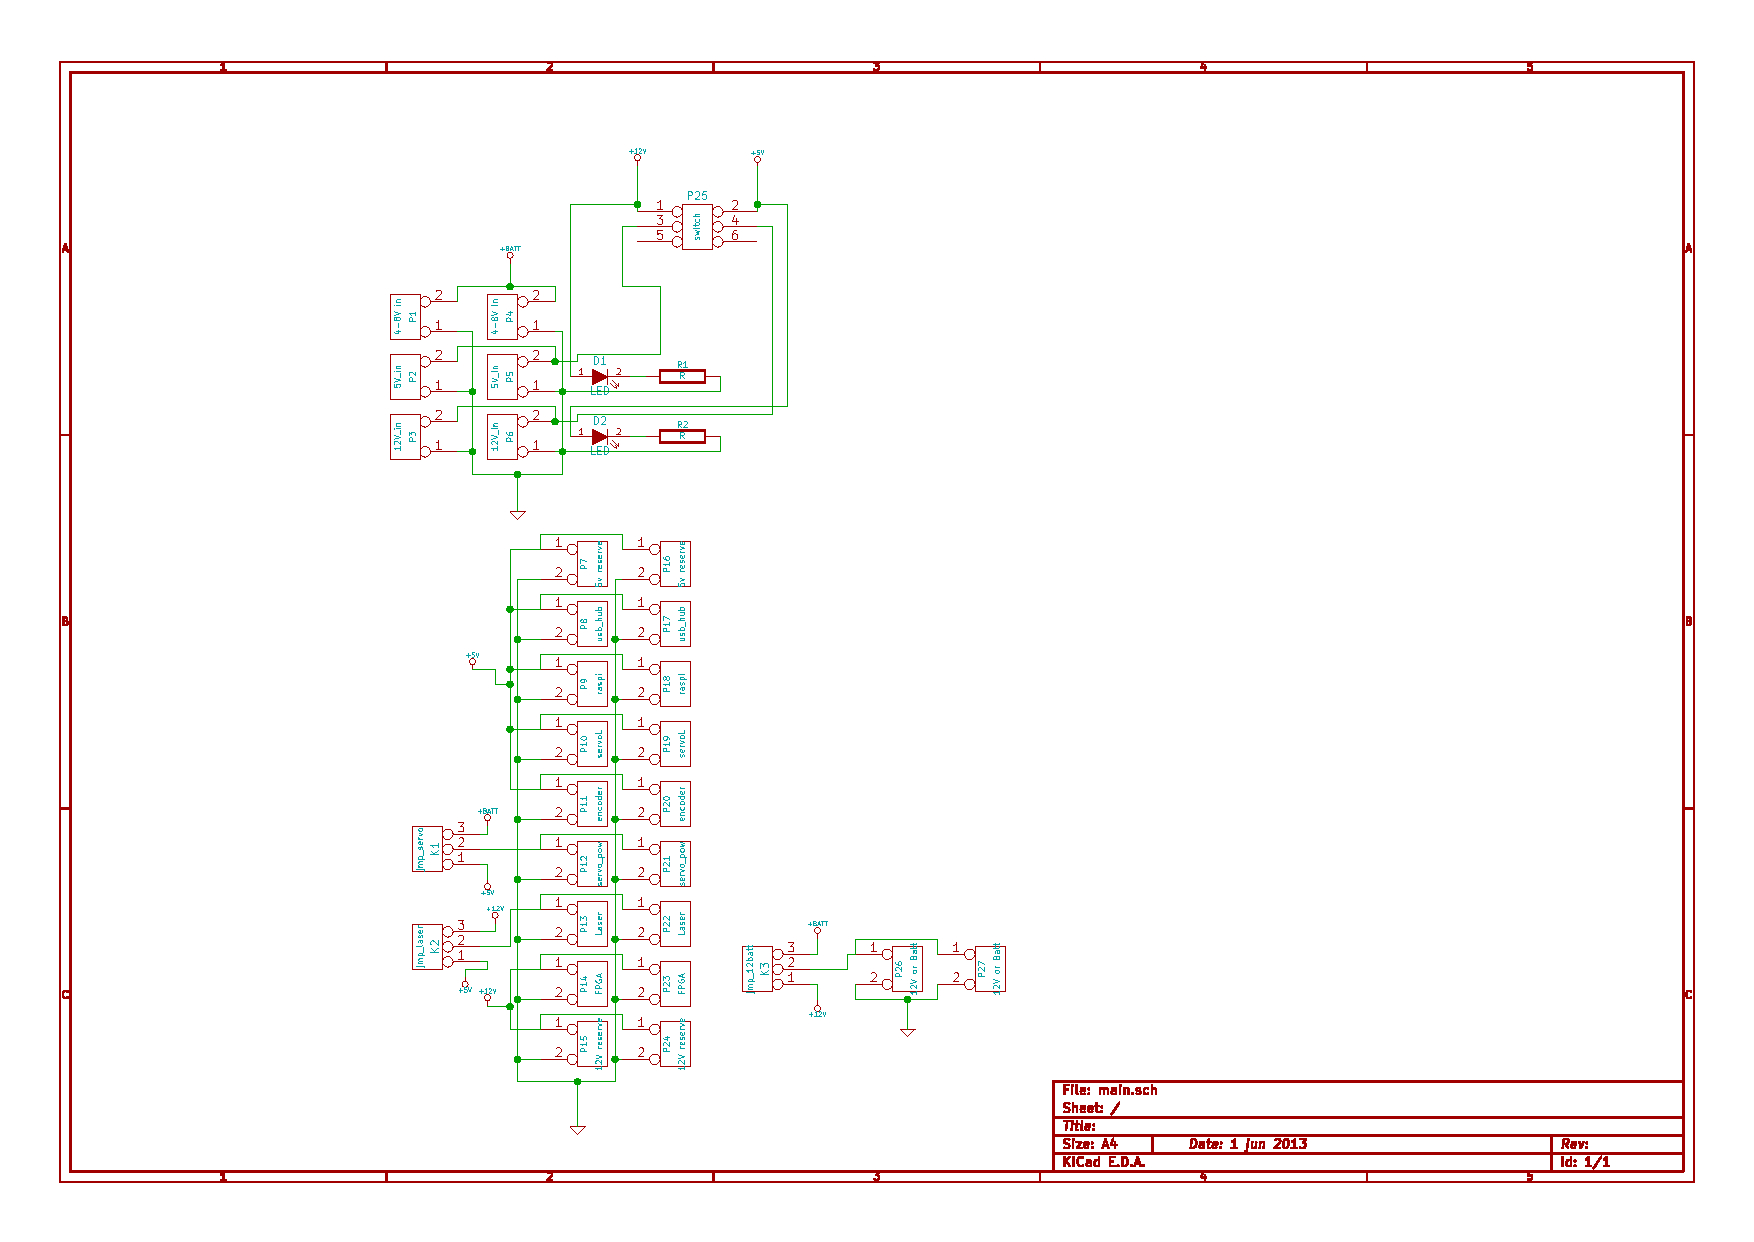
\includegraphics[width=20cm,angle=-90]{pic/powerboard}
\caption{Powerboard schematics}
\end{center}
\label{figpowerboardscm}
\end{figure}

\begin{figure}[h]
\begin{center}
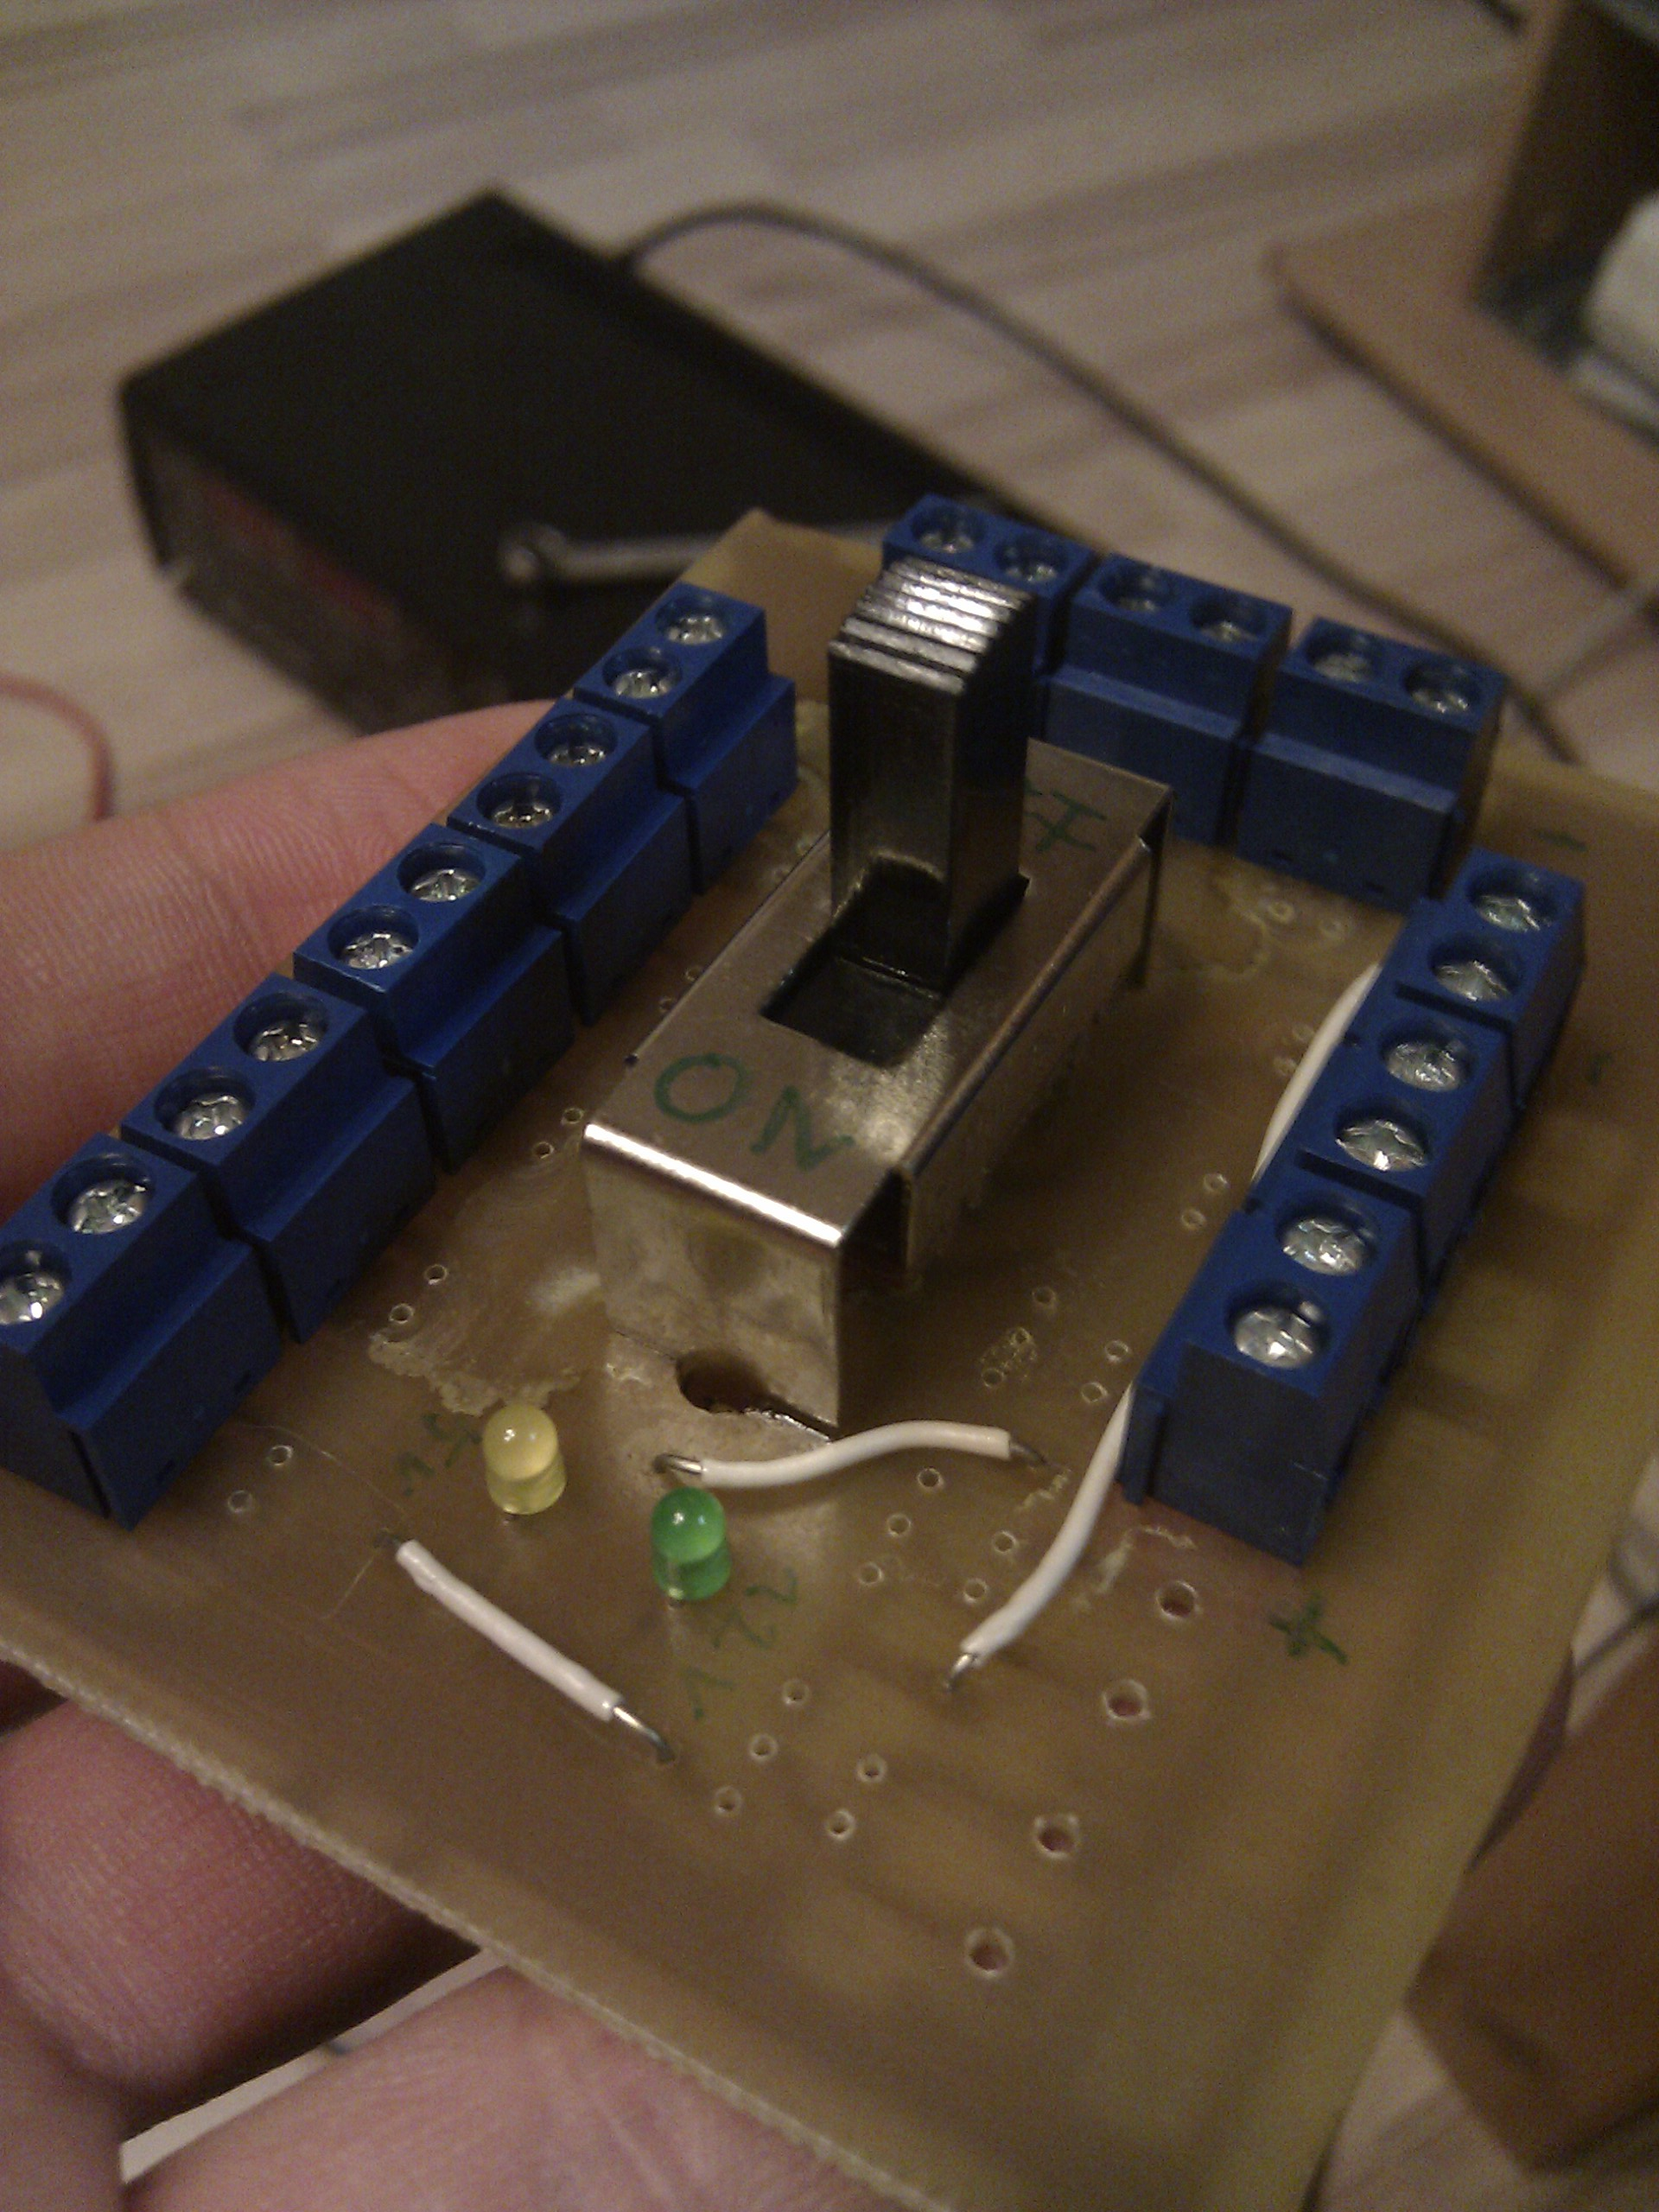
\includegraphics[width=8cm]{pic/powerboardr.jpg}
\caption{Powerboard}
\end{center}
\label{figpowerboardr}
\end{figure}


\section{Rotary Encoders} %%TODO: richtige bezeichnung???

To measure speed, we built two rotary encoders into the car.
They are based on a simple and cheap light barrier with an included Schmitt trigger and a rotary encoder disc.
There are four 



To connect the light barriers to the FPGA, we built a sensorboard. It has the task to supply the light barriers with power and to convert the output voltage of the light barriers to the right level.
There are also two LEDs on the board, that show the current state of the light barriers.
This made it easier to debug the light barriers when moving the rotary encoder discs into position.
The schematics of the sensorboard can be seen in Figure \ref{figsensorboardscm}. The board layout and a 3D rendering can be seen in Figures \ref{figsensorboardbrd} and \ref{figsensorboard3d}.

\begin{figure}[htb]
\begin{center}
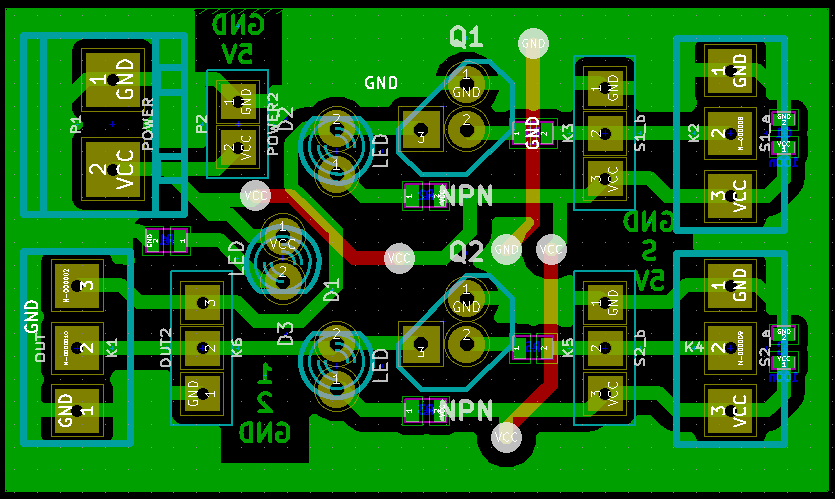
\includegraphics[width=8cm]{pic/sensorboardbrd.png}
\caption{Sensorboard}
\end{center}
\label{figsensorboardbrd}
\end{figure}

\begin{figure}[htb]
\begin{center}
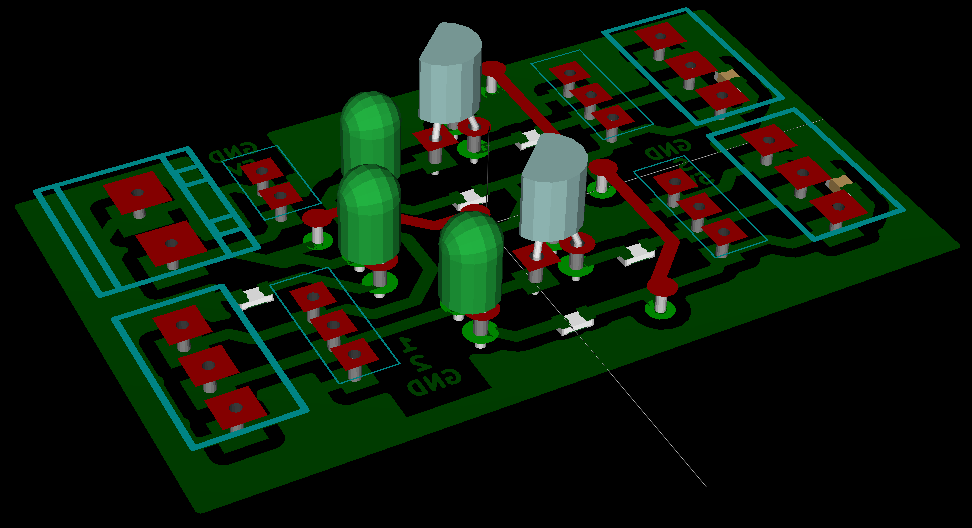
\includegraphics[width=8cm]{pic/sensorboard3d.png}
\caption{Sensorboard}
\end{center}
\label{figsensorboard3d}
\end{figure}

\begin{figure}[htb]
\begin{center}
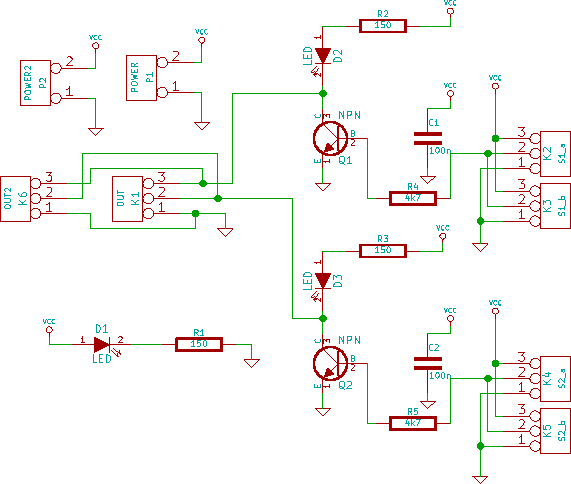
\includegraphics[width=20cm,angle=-90]{pic/sensorboard}
\caption{Sensorboard schematics}
\end{center}
\label{figsensorboardscm}
\end{figure}


\section{Conclusions}\label{conclusions}
We worked hard, and achieved very little.

\section{Future work}

\bibliographystyle{abbrv}
\bibliography{doku}

\end{document}
